\documentclass{llncs}
\pagestyle{plain}
\usepackage{amsmath,amssymb,amsfonts,stmaryrd}
\usepackage{graphicx}
\usepackage[usenames,dvipsnames]{color}
\usepackage{tikz}
\usepackage{hyperref}
\usepackage[T1]{fontenc}
\usepackage{listings}
\usepackage{booktabs}
\lstset{%
   basicstyle=\ttfamily, %\scriptsize\ttfamily,
%   frame=single,
   breaklines=true,
}
%\usepackage{algorithm}
\usepackage{float}

\newcommand{\wip}[1]{\textcolor{Purple}{WIPWIPWIPWIP #1 WIPWIPWIPWIP}}

\newif\ifcomments

\commentstrue
%\commentsfalse

\newcommand{\francois}[1]{\ifcomments  \textcolor{blue}{#1}\fi}
\newcommand{\sylvain}[1]{\ifcomments \textcolor{green}{#1} \fi}
\newcommand{\arthur}[1]{\ifcomments \textcolor{brown}{#1} \fi}


\newcommand{\defleq}{\sqsubseteq_{\text{def}}}
\newcommand{\lra}{\longrightarrow}

\floatstyle{boxed}
\newfloat{listfig}{htb}{lstfig}
\floatname{listfig}{Listing}

\floatstyle{ruled}
\newfloat{algorithm}{htpb}{algfig}
\floatname{algorithm}{Algorithm}




\begin{document}

\title{PAC Learning of Thomas Regulatory Networks from Time-Series Data}

\author{Arthur Carcano\inst{1} \and Fran\c{c}ois Fages\inst{2} \and J\'er\'emy Grignard\inst{2} \and Sylvain
Soliman\inst{2}}

\institute{%
Ecole Normale Sup\'erieure, Paris, France\\
  \email{arthur.carcano@ens.fr}
\and Inria, University Paris-Saclay, Lifeware group, France\\
   \email{Francois.Fages@inria.fr},
   \email{Sylvain.Soliman@inria.fr}
}

\maketitle

\begin{abstract}
Automating the process of model building from experimental data 
is a very desirable goal to palliate the lack of modellers for many applications.
However, despite the spectacular progress of machine learning techniques in data analytics, classification, clustering and prediction making,
learning dynamical models from data time-series is still challenging.
In this paper we investigate the use of the Probably Approximately Correct (PAC) learning 
framework of Leslie Valiant as a method for the automated discovery of influence models of biochemical processes from Boolean and stochastic traces. 
We show that Thomas' Boolean influence systems can be naturally represented by k-CNF formulae
and learned
from time-series data with a quasi linear number of Boolean activation samples per species,
and that positive Boolean influence systems can be represented by monotone DNF formulae
and learned actively with both activation samples and oracle calls.
We evaluate the performance of this approach on a model of T-lymphocyte
differentiation, with and without prior knowledge,
and discuss its merits as well as its limitations with respect to realistic experiments.
\end{abstract}

\section{Introduction}

Modelling biological systems is still an art which is currently limited in its applications by the number of available modellers.
Automating the process of model building is thus a very desirable goal
to attack new applications, develop patient-tailored therapeutics,
and also design experiments that can now be largely automated
with a gain in both the quantification and the reliability of the observations, at both the single cell and population levels.

Machine learning is revolutionising the statistical methods in biological data analytics,
data classification and clustering, and prediction making.
However, learning dynamical models from data time-series is still challenging.
A recent survey on probabilistic programming \cite{GHNR14fose}
highlighted the difficulties associated with modelling time,
and concluded that existing frameworks are not sufficient in their treatment of dynamical systems.
There has been early work on the use of machine learning techniques, such as inductive
 logic programming~\cite{Muggleton95ngc} combined with active learning in the vision of the ``robot scientist''~\cite{BMOKRK01etai},
to infer gene functions,
metabolic pathway descriptions~\cite{AM02etai,AM02slps}
or gene influence systems~\cite{BCRG04jtb},
or to revise a reaction model with respect to CTL properties~\cite{CCFS06tcsb}.
Since a few years, progress in this field is measured on public benchmarks
of the ``Dream Challenge'' competition~\cite{Meyer14bmc}.
Logic Programming, and especially \emph{Answer Set Programming} (ASP), provide efficient tools such as CLASP~\cite{GKNS07lpnmr}
to implement learning algorithms for Boolean models.
They have been applied in~\cite{GSTUV08iclp} to the detection of  inconsistencies in large biological networks,
and have been subsequentially applied to the inference of gene networks from gene expression data and to the design of discriminant experiments~\cite{VKASSSG15frontiers}.
Furthermore, ASP has been combined with CTL model-checking in~\cite{OPSSG16biosystems} to learn mammalian signalling networks from time series data,
and identify erroneous time-points in the data.

%Active learning extends machine learning with the possibility to call oracles, e.g.~make experiments,
%and budgeted learning adds costs to the calls to the oracle.
%The original motivation for the budgeted learning protocol came from medical applications in which the outcome of a treatment,
%drug trial, or control group is known, and the results of running medical tests are each available for a price~\cite{DZBSM13ml}.
%In this context, multi-armed bandit methods~\cite{DBSSZ07icdm} currently provide the best strategies.
%In~\cite{LMALS14ecml}, a bandit-based active learning algorithm is proposed for experiment design in dynamical system identification.

In this paper, we consider the framework of Probably Approximately Correct (PAC) Learning 
which was introduced by Leslie Valiant in his seminal paper on a theory of the learnable~\cite{Valiant84cacm}.
Valiant questioned what can be learned from a computational viewpoint,
and introduced the concept of PAC learning,
together with a general-purpose polynomial-time learning protocol.
Beyond the algorithms that one can derive with this methodology,
Valiant's theory of the learnable has profound implications
on the nature of biological and cognitive processes,
of collective and individual behaviors,
and on the study of their evolution~\cite{Valiant13book}.

Here we investigate PAC learning as a method for the automated discovery of influence models of biochemical processes from time-series data. 
To the best of our knowledge, 
the application of PAC learning to dynamical models of biochemical systems has not been reported before.
We show that Thomas' gene regulatory networks~\cite{Thomas91jtb,Thomas73jtb} can be naturally represented by 
Boolean formulae in conjunctive normal forms with a bounded number of litterals (i.e.~k-CNF formulae),
and can be learned from Boolean transitions with a quasi linear number of Boolean transition samples, using Valiant's PAC learning algorithm for k-CNF formulae.
We also show that Boolean influence systems with their positive Boolean semantics discussed in~\cite{FMRS16cmsb}
can be naturally represented by monotone DNF formulae,
and learned actively from a set of positive samples with calls to an oracle.
These results\footnote{The code is available at \url{http://lifeware.inria.fr/wiki/software/\#CMSB17}.} 
are evaluated on a Boolean influence model of 
the differentiation of the T-helper lymphocytes from \cite{RRMTC06tcsb,Mendoza06biosystems},
composed of 32 influences and 12 variables.


\section{Valiant's PAC Learning Algorithms}\label{pac}


%\subsection{PAC Learning Protocol}

Let $n$ be the dimension of the model to learn, and let us consider a finite set of Boolean variables $x_1,\ldots,x_n$,
 A vector is an assignment of the $n$ variables to $\mathbb{B}_* = \{0,1,*\}$;
 A total vector is a Boolean assignment, in $\mathbb{B} = \{0,1\}$;
 A Boolean function $G:{\mathbb{B}}^n \rightarrow \mathbb{B}$;
	assigns a Boolean value to each total vector;
 A concept $F:{\mathbb{B}_*}^n \rightarrow \mathbb{B}$
	assigns a Boolean value to each vector.

The idea behind the PAC learning protocol is to discover a concept, or a Boolean function, $G$ which approximates a hidden concept $F$, while restricting oneself to the two following operations~:
\begin{itemize}
  \item
\textsc{Sample}$()$: returns a positive example, i.e.~a vector $v$ such that $F(v)=1$.
The output of \textsc{Sample}$()$ is assumed to follow a given probability distribution $D(v)$, which is used to measure the approximation of the result.
  \item
\textsc{Oracle}$(v)$: returns the value of $F(v)$ for any input vector $v$.
\end{itemize}


\begin{definition}[\cite{Valiant84cacm}]\label{def:learnclass}
   A class $\cal M$ of \emph{Boolean functions} is said to be \emph{learnable}
   if there exists an algorithm $\cal A$ with some precision parameter $h\in\mathbb N$ such that
$\cal A$ runs in polynomial time both in $n$ and $h$;
and         for any function $F$ in $\cal M$, and any distribution $D$ on the positive examples,
         $\cal A$ deduces with probability higher than $1-h^{-1}$ an approximation $G$ of $F$ such that
         \begin{itemize}
            \item $G(v)=1$ implies $F(v)=1$ (no false positive)
            \item
               $\displaystyle\sum_{v\ s.t.\ F(v)=1\wedge G(v)=0} D(v) < h^{-1}$ (low probability of false negatives)
         \end{itemize}
\end{definition}


Valiant showed the learnability of some important classes of functions in this framework,
in particular for Boolean formulae in conjunctive normal forms with at most $k$ literals per conjunct (k-CNF),
and for monotone (i.e.~negation free) Boolean formulae in disjunctive normal form (DNF).
The computational complexities of the PAC learning algorithms are expressed in terms of some function


\begin{theorem}[\cite{Valiant84cacm}]\label{thm:kcnf}\label{thm:mdnf}
For any $k$, the class of $k$-CNF formulae (i.e.~with at most $k$ literals per conjunct) on $n$ variables is learnable with an
algorithm that uses $L(h,{(2 n)}^{k+1})$ positive examples and no call to the
oracle (where $L(h,S) \le 2h(S+\log_e h)$).
The class of monotone (i.e.~without negation) DNF formulae on $n$ variables is also learnable with an
algorithm that uses $L(h,d)$ examples and $d n$ calls to the oracle
(where $d$ is the largest number of prime
implicants in an equivalent rewriting of the formula to learn as a non-redundant sum of
prime-implicants).
\end{theorem}


\section{Thomas's Boolean Regulatory Network}


\begin{definition}[\cite{Thomas73jtb}]
   A \emph{Thomas} network on a finite set of genes $\{x_1,\dots,x_n\}$
   is defined by  $n$ Boolean functions $\{f_1,\dots,f_n\}$ which give for each gene its
   possible next state, given the current state.
\end{definition}



$k$-CNF formulae can be used to represent Thomas gene regulatory network functions with some reasonable restrictions on their connectivity,
e.g.~for networks of degree bounded by $k$,
When restricting to monotone activation functions, i.e.~without negation testing the absence of expression of a gene,
monotone DNF formulae can be used as well to represent monotone Thomas networks, i.e.~with positive and negative influences but no influence inhibitors \cite{FMRS16cmsb}.

\noindent
\begin{minipage}{0.5\textwidth}
Here we consider a regulatory network of 12 variables which models the  differentiation between Th-1 and Th-2 lymphocytes from an original
CD4+ T helper (Th-0).
The model has three different stable states corresponding to Th-0 (naive
lymphocyte), Th-1 and Th-2 when IL12 is off, and two others when IL12 is on
(the Th-0 one is lost).
This model, presented in~\cite{RRMTC06tcsb} is actually a Boolean
simplification of the original multi-level model
of~\cite{Mendoza06biosystems}. 
\end{minipage}
\begin{minipage}{0.5\textwidth}
   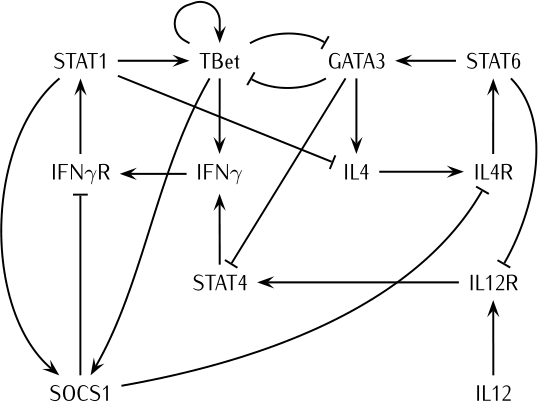
\includegraphics[width=\textwidth]{th_net_clean.png}
\end{minipage}

\section{PAC Learning from Boolean and Stochastic Traces}
\label{sec:abinitio}



Valiant's work on PAC learning provides an elegant trail 
to attack the challenge of inferring the structure of influence models from the observation of data time series,
and more precisely to automatically discover possible regulatory networks of a biochemical process, given sufficiently precise observations of its executions.

The Boolean dynamics of biochemical influence systems, including Thomas regulatory networks, can be represented by $k$-CNF formulae without loss of generality,
and $k$-CNF PAC learning algorithm can be used to infer the strucutre of the network from
a sufficiently large and diverse set of state transition traces.
When dimension increases, we show on the example of T-lymphocyte differentiation from the litterature
that the $k$-CNF PAC learning algorithm can also leverage available
prior knowledge on the system to deliver precise results with a reasonable
amount of data.

The Boolean dynamics of positive influence systems can also be straightforwardly represented by monotone DNF activation and deactivation functions,
and monotone DNF PAC learning algorithm applied with an interesting recourse to oracles 
which are particularly relevant in the perspective of online active learning and experimental design.

More work is needed however to make comparisons on common benchmarks
with  other approaches already investigated in this context, such as Answer Set Programming (ASP) and budgeted learning,
and to investigate the applicability of these methods to real experiments taking into account particular biological technologies.

\bibliographystyle{splncs03}
\bibliography{contraintes}
\end{document}

